\section{Challenges and Open Problems}

% ---------------------------------------------------------------- Slide 27 (divider)
\begin{frame}{}
    \LARGE Challenges and \textbf{Open Problems} in RL
\end{frame}

% ---------------------------------------------------------------- Slide 29
\begin{frame}{What's the problem?}
\textbf{Challenges with core algorithms:}
\begin{itemize}
    \item \textbf{Stability:} does your algorithm converge?
    \item \textbf{Efficiency:} how long does it take to converge? (how many samples)
    \item \textbf{Generalization:} after it converges, does it generalize?
\end{itemize}
\vspace{0.8em}
\textbf{Challenges with assumptions:}
\begin{itemize}
    \item Is this even the right problem formulation?
    \item What is the source of supervision?
\end{itemize}
\end{frame}

% ---------------------------------------------------------------- Slide 30
\begin{frame}[shrink=12]{Stability and hyperparameter tuning}
\begin{columns}[c]
\begin{column}{0.72\textwidth}
\begin{itemize}
    \item Devising stable RL algorithms is very hard
    \item Q-learning / value function estimation
    \begin{itemize}
        \item Fitted Q / fitted value methods with deep network function estimators are
              typically not contractions, hence no guarantee of convergence
        \item Lots of parameters for stability: target network delay, replay buffer
              size, clipping, sensitivity to learning rates, etc.
    \end{itemize}
    \item Policy gradient / likelihood ratio / REINFORCE
    \begin{itemize}
        \item Very high variance gradient estimator
        \item Lots of samples, complex baselines, etc.
        \item Parameters: batch size, learning rate, design of baseline
    \end{itemize}
    \item Model-based RL algorithms
    \begin{itemize}
        \item Model class and fitting method
        \item Optimizing policy w.r.t.\ model non-trivial due to backpropagation through time
        \item More subtle issue: policy tends to exploit the model
    \end{itemize}
\end{itemize}
\end{column}
\begin{column}{0.28\textwidth}
\centering
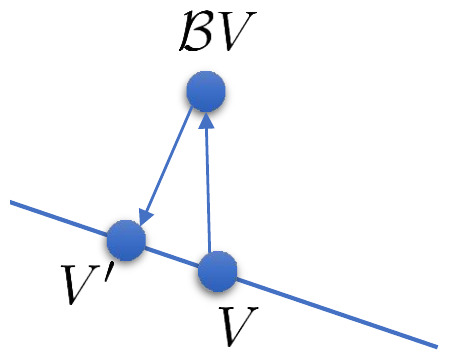
\includegraphics[width=\linewidth]{images/meta-rl-open/figures/bellman-fig.jpg}
\end{column}
\end{columns}
\end{frame}

% ---------------------------------------------------------------- Slide 31
\begin{frame}{The challenge with sample complexity}
\begin{columns}[c]
\begin{column}{0.6\textwidth}
\begin{itemize}
    \item Need to wait for a long time for your homework to finish running
    \item Real-world learning becomes difficult or impractical
    \item Precludes the use of expensive, high-fidelity simulators
    \item Limits applicability to real-world problems
\end{itemize}
\end{column}
\begin{column}{0.4\textwidth}
\centering

\includegraphics[width=0.66\linewidth]{images/meta-rl-open/figures/atari-homework.jpg}\\[0.5em]
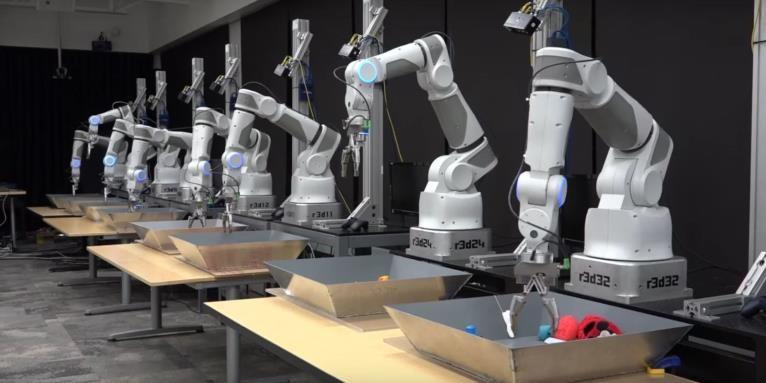
\includegraphics[width=\linewidth]{images/meta-rl-open/figures/sample-complexity.jpg}
\end{column}
\end{columns}
\end{frame}

% ---------------------------------------------------------------- Slide 32
\begin{frame}{Scaling up deep RL \& generalization}
\begin{columns}[c]
\begin{column}{0.42\textwidth}
\centering
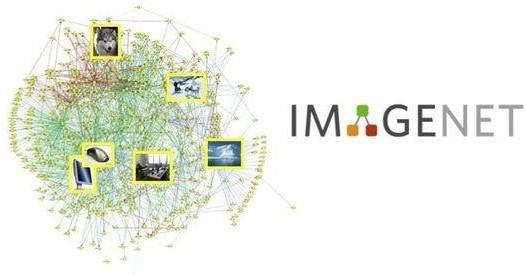
\includegraphics[width=0.95\linewidth]{images/meta-rl-open/figures/imagenet-collage.jpg}\\[0.8em]
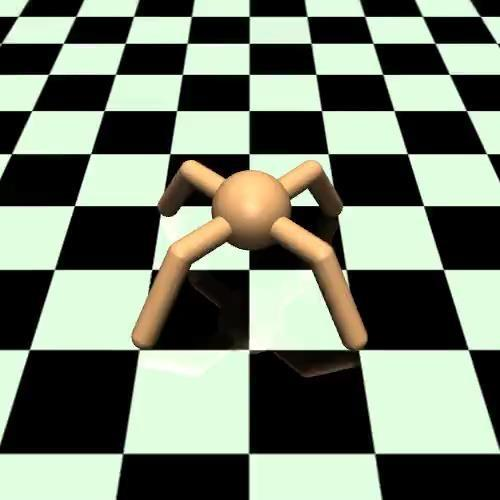
\includegraphics[width=0.52\linewidth]{images/meta-rl-open/figures/chess-board.jpg}
\end{column}
\begin{column}{0.58\textwidth}
\begin{itemize}
    \item Large-scale
    \item Emphasizes diversity
    \item Evaluated on generalization
\end{itemize}
\vspace{1.6em}
\begin{itemize}
    \item Small-scale
    \item Emphasizes mastery
    \item Evaluated on performance
    \item Where is the generalization?
\end{itemize}
\end{column}
\end{columns}
\end{frame}

% ---------------------------------------------------------------- Slide 33
\begin{frame}{RL has a big problem}
\vfill
\centering
\resizebox{\textwidth}{!}{%
\begin{tikzpicture}[
   ic/.style={inner sep=0},
   txt/.style={align=center, font=\footnotesize},
   ga/.style={-{Stealth[length=4mm]}, line width=3.5pt, green!50!black},
   ba/.style={-{Stealth[length=3mm]}, line width=2.5pt, blue!55!black}]
   \node[font=\normalsize] at (2.4,3.1) {reinforcement learning};
   \node[font=\normalsize] at (9.3,3.1) {supervised machine learning};
   % --- left: RL loop ---
   \node[ic] (e1) at (0.9,0.7) {
\includegraphics[height=1.5cm]{images/meta-rl-open/figures/icons/earth.jpg}};
   \node[ic] (r1) at (3.2,1.9) {
\includegraphics[height=1.4cm]{images/meta-rl-open/figures/icons/robot.jpg}};
   \node[ic] (n1) at (3.7,-0.3) {
\includegraphics[height=1.0cm]{images/meta-rl-open/figures/icons/nn.jpg}};
   \node[txt] at (2.85,0.45) {this is done\\\textbf{many times}};
   \draw[ga] (e1) to[bend left=45] (r1);
   \draw[ga] (r1) to[bend left=25] (n1);
   \draw[ga] (n1) to[bend left=45] (e1);
   % --- right: supervised (earth -> dataset -> net -> robot) ---
   \node[ic] (e2) at (7.0,2.1) {
\includegraphics[height=1.3cm]{images/meta-rl-open/figures/icons/earth.jpg}};
   \node[ic] (d2) at (9.7,2.1) {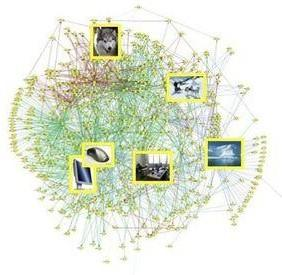
\includegraphics[height=1.5cm]{images/meta-rl-open/figures/icons/dataset.jpg}};
   \node[txt] at (8.35,1.35) {this is done\\\textbf{once}};
   \node[ic] (n2) at (9.7,0.2) {
\includegraphics[height=1.1cm]{images/meta-rl-open/figures/icons/nn.jpg}};
   \node[ic] (r2) at (9.7,-1.7) {
\includegraphics[height=1.4cm]{images/meta-rl-open/figures/icons/robot.jpg}};
   \node[txt] at (11.95,1.05) {train for\\\textbf{many epochs}};
   \draw[ga] (e2) to[bend left=35] (d2);
   \draw[ga] (d2) -- (n2);
   \draw[ba, -{Stealth[length=2.8mm]}] ([shift={(10.85,1.05)}]65:0.36) arc[start angle=65, end angle=-255, radius=0.36];
   \draw[ga] (n2) -- (r2);
\end{tikzpicture}}
\vfill
\end{frame}

% ---------------------------------------------------------------- Slide 34
\begin{frame}{RL has a big problem}
\vfill
\centering
\begin{tikzpicture}[
   ic/.style={inner sep=0},
   txt/.style={align=center, font=\footnotesize},
   ga/.style={-{Stealth[length=4mm]}, line width=3.5pt, green!50!black}]
   \node[font=\normalsize] at (2.4,3.55) {reinforcement learning};
   \node[font=\normalsize] at (9.4,3.55) {actual reinforcement learning};
   % --- left: RL loop ---
   \node[ic] (e1) at (0.9,0.7) {
\includegraphics[height=1.5cm]{images/meta-rl-open/figures/icons/earth.jpg}};
   \node[ic] (r1) at (3.2,1.9) {
\includegraphics[height=1.4cm]{images/meta-rl-open/figures/icons/robot.jpg}};
   \node[ic] (n1) at (3.7,-0.3) {
\includegraphics[height=1.0cm]{images/meta-rl-open/figures/icons/nn.jpg}};
   \node[txt] at (2.85,0.45) {this is done\\\textbf{many times}};
   \draw[ga] (e1) to[bend left=45] (r1);
   \draw[ga] (r1) to[bend left=25] (n1);
   \draw[ga] (n1) to[bend left=45] (e1);
   % --- right: inner loop inside a box ---
   \node[ic] (e2) at (7.4,1.7) {
\includegraphics[height=1.2cm]{images/meta-rl-open/figures/icons/earth.jpg}};
   \node[ic] (r2) at (9.2,2.4) {
\includegraphics[height=1.1cm]{images/meta-rl-open/figures/icons/robot.jpg}};
   \node[ic] (n2) at (10.7,1.3) {
\includegraphics[height=0.85cm]{images/meta-rl-open/figures/icons/nn.jpg}};
   \node[txt] at (8.9,1.3) {this is done\\\textbf{many times}};
   \draw[ga] (e2) to[bend left=40] (r2);
   \draw[ga] (r2) to[bend left=22] (n2);
   \draw[ga] (n2) to[bend left=40] (e2);
   \node[draw, rounded corners, fit=(e2)(r2)(n2), inner sep=8pt] (box) {};
   % --- outer loop to person ---
   \node[ic] (p2) at (9.0,-2.0) {
\includegraphics[height=1.3cm]{images/meta-rl-open/figures/icons/person.jpg}};
   \node[txt] at (9.0,-0.7) {this is done\\\textbf{many many times}};
   \draw[ga] (box.east) to[bend left=35] (p2.east);
   \draw[ga] (p2.west) to[bend left=35] (box.west);
\end{tikzpicture}
\vfill
\end{frame}

% ---------------------------------------------------------------- Slide 35
\begin{frame}{How bad is it?}
\begin{columns}[c]
\begin{column}{0.46\textwidth}
\centering
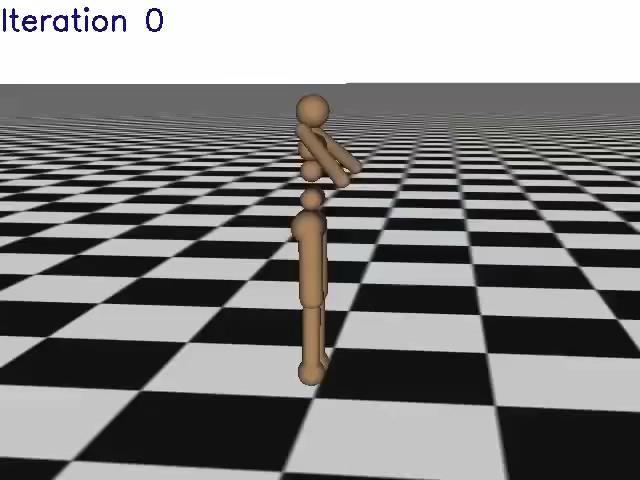
\includegraphics[width=\linewidth]{images/meta-rl-open/figures/humanoid-iter.jpg}
\end{column}
\begin{column}{0.54\textwidth}
\begin{itemize}
    \item This is quite cool
    \item It takes 6 days of real time (if it was real time)
    \item \dots to run on an infinite flat plane
\end{itemize}
\vspace{0.3em}
\begin{center}
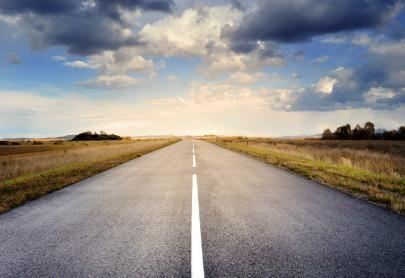
\includegraphics[width=0.36\linewidth]{images/meta-rl-open/figures/rw-road.jpg}\;%
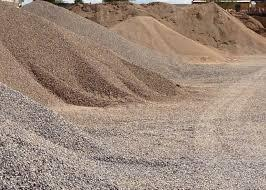
\includegraphics[width=0.36\linewidth]{images/meta-rl-open/figures/rw-desert.jpg}\\[0.3em]
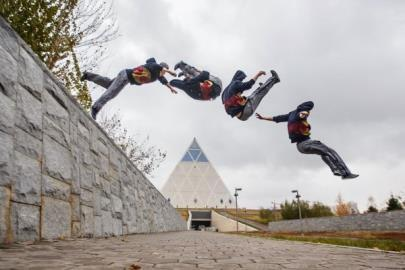
\includegraphics[width=0.36\linewidth]{images/meta-rl-open/figures/rw-parkour.jpg}\;%
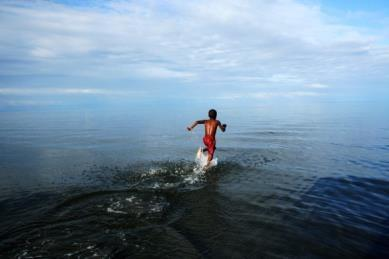
\includegraphics[width=0.36\linewidth]{images/meta-rl-open/figures/rw-person.jpg}
\end{center}
\textbf{The real world is not so simple!}
\end{column}
\end{columns}
\vfill
{\scriptsize Schulman, Moritz, L., Jordan, Abbeel '16}
\end{frame}

% ---------------------------------------------------------------- Slide 36
\begin{frame}{Off-policy RL?}
\vfill
\centering
\resizebox{\textwidth}{!}{%
\begin{tikzpicture}[
   ic/.style={inner sep=0},
   txt/.style={align=center, font=\footnotesize},
   ga/.style={-{Stealth[length=4mm]}, line width=3.5pt, green!50!black},
   ba/.style={-{Stealth[length=3mm]}, line width=2.5pt, blue!55!black}]
   \node[font=\normalsize] at (2.4,3.2) {reinforcement learning};
   \node[font=\normalsize] at (9.4,3.2) {off-policy reinforcement learning};
   % --- left: RL loop ---
   \node[ic] (e1) at (0.9,0.7) {
\includegraphics[height=1.5cm]{images/meta-rl-open/figures/icons/earth.jpg}};
   \node[ic] (r1) at (3.2,1.9) {
\includegraphics[height=1.4cm]{images/meta-rl-open/figures/icons/robot.jpg}};
   \node[ic] (n1) at (3.7,-0.3) {
\includegraphics[height=1.0cm]{images/meta-rl-open/figures/icons/nn.jpg}};
   \node[txt] at (2.85,0.45) {this is done\\\textbf{many times}};
   \draw[ga] (e1) to[bend left=45] (r1);
   \draw[ga] (r1) to[bend left=25] (n1);
   \draw[ga] (n1) to[bend left=45] (e1);
   % --- right: off-policy ---
   \node[ic] (e2) at (7.0,0.9) {
\includegraphics[height=1.3cm]{images/meta-rl-open/figures/icons/earth.jpg}};
   \node[ic] (r2) at (8.3,2.2) {
\includegraphics[height=1.1cm]{images/meta-rl-open/figures/icons/robot.jpg}};
   \node[ic] (d2) at (9.6,1.7) {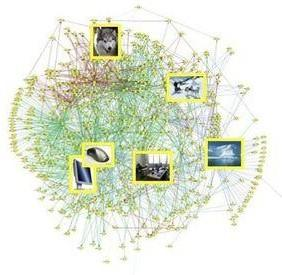
\includegraphics[height=1.1cm]{images/meta-rl-open/figures/icons/dataset.jpg}};
   \node[txt] at (9.6,0.55) {big dataset from\\ past interaction};
   \node[ic] (n2) at (11.0,1.7) {
\includegraphics[height=0.85cm]{images/meta-rl-open/figures/icons/nn.jpg}};
   \node[txt] at (11.9,0.55) {train for\\\textbf{many epochs}};
   \node[ic] (p2) at (11.0,-1.7) {
\includegraphics[height=1.2cm]{images/meta-rl-open/figures/icons/person.jpg}};
   \node[txt] at (7.5,-1.6) {occasionally\\ get more data};
   \draw[ga] (e2) to[bend left=35] (r2);
   \draw[ga] (r2) to[bend left=15] (d2);
   \draw[ga] (d2) -- (n2);
   \draw[ba, -{Stealth[length=2.8mm]}] ([shift={(11.9,1.7)}]65:0.32) arc[start angle=65, end angle=-255, radius=0.32];
   \draw[ga] (n2) -- (p2);
   \draw[ga] (p2) to[bend left=20] (e2);
\end{tikzpicture}}
\vfill
\end{frame}

% ---------------------------------------------------------------- Slide 37
\begin{frame}{Single task or multi-task?}
\begin{columns}[c]
\begin{column}{0.3\textwidth}
\centering
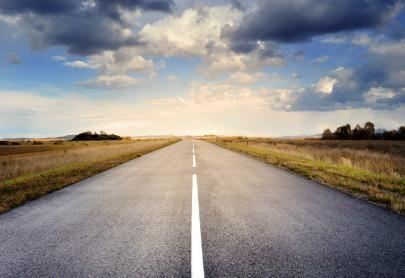
\includegraphics[width=0.46\linewidth]{images/meta-rl-open/figures/rw-road.jpg}\,%
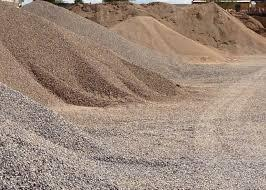
\includegraphics[width=0.46\linewidth]{images/meta-rl-open/figures/rw-desert.jpg}\\[0.3em]
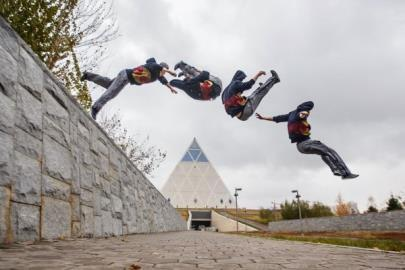
\includegraphics[width=0.46\linewidth]{images/meta-rl-open/figures/rw-parkour.jpg}\,%
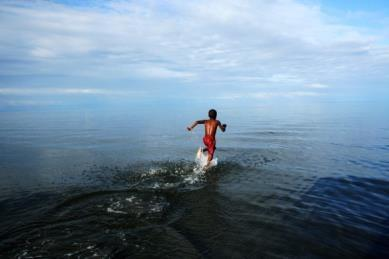
\includegraphics[width=0.46\linewidth]{images/meta-rl-open/figures/rw-person.jpg}
\end{column}
\begin{column}{0.7\textwidth}
\begin{itemize}
    \item this is where generalization can come from\dots
    \item maybe doesn't require any new assumption, but might merit additional treatment
\end{itemize}
\end{column}
\end{columns}
\vspace{0.4em}
\textbf{The real world is not so simple!}
\vfill
\begin{center}
\begin{tikzpicture}[font=\footnotesize, >={Stealth[length=1.6mm]}]
    \node[align=center] (pick) at (0,0) {pick MDP randomly\\ in first state};
    \node (ps) at (2.5,0) {$p(s_0)$};
    \node[anchor=west] (r0) at (4.0,0.85)  {$s_0 \xrightarrow{\;\pi(a_0|s_0)\;} s_1 \longrightarrow$ \;etc.\quad MDP 0};
    \node[anchor=west] (r1) at (4.0,0.0)   {$s_0 \xrightarrow{\;\pi(a_0|s_0)\;} s_1 \longrightarrow$ \;etc.\quad MDP 1};
    \node[anchor=west] (r2) at (4.0,-0.85) {$s_0 \xrightarrow{\;\pi(a_0|s_0)\;} s_1 \longrightarrow$ \;etc.\quad MDP 2};
    \draw[->] (ps) -- node[above,font=\tiny,sloped]{sample} (r0.west);
    \draw[->] (ps) -- node[above,font=\tiny]{sample} (r1.west);
    \draw[->] (ps) -- node[below,font=\tiny,sloped]{sample} (r2.west);
\end{tikzpicture}
\end{center}
\end{frame}

% ---------------------------------------------------------------- Slide 38
\begin{frame}{Where does the supervision come from?}
\begin{columns}[c]
\begin{column}{0.55\textwidth}
\begin{itemize}
    \item If you want to learn from many different tasks, you need to get those tasks
          somewhere!
    \item Learn objectives / rewards from demonstration (inverse reinforcement learning)
    \item Generate objectives automatically?
\end{itemize}
\end{column}
\begin{column}{0.45\textwidth}
\centering
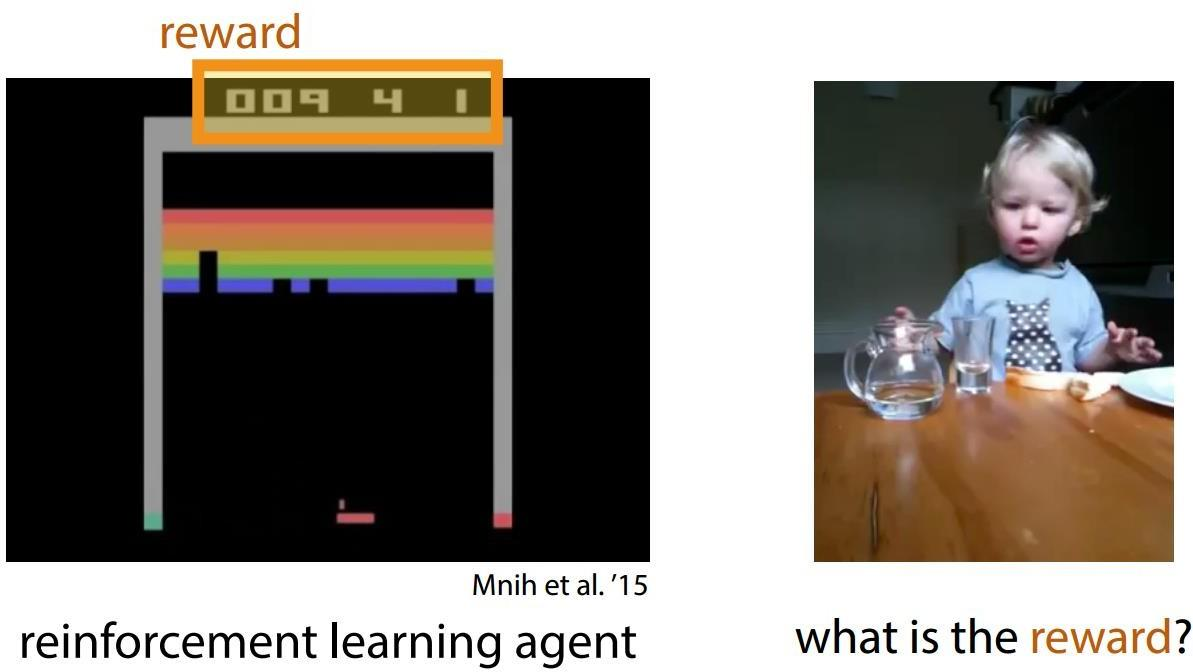
\includegraphics[width=\linewidth,height=0.7\textheight,keepaspectratio]{images/meta-rl-open/figures/supervision.jpg}
\end{column}
\end{columns}
\end{frame}

% ---------------------------------------------------------------- Slide 39
\begin{frame}{Rethinking the Problem Formulation}
\begin{itemize}
    \item How should we define a control problem?
    \begin{itemize}
        \item What is the data?
        \item What is the goal?
        \item What is the supervision? \quad{\footnotesize(may not be the same as the goal\dots)}
    \end{itemize}
    \item Think about the assumptions that fit your problem setting!
    \item Don't assume that the basic RL problem is set in stone
\end{itemize}
\end{frame}
